% =====================================================================
%  PULSE --- v2 of the overview: what changed in October, what it bought,
%  what is next. Same look as pulse-overview.tex.
%  Compile:  pdflatex pulse-overview-v2.tex
% =====================================================================
\documentclass[10pt,a4paper]{article}
\usepackage[utf8]{inputenc}
\usepackage[T1]{fontenc}
\usepackage{lmodern}
\usepackage{microtype}
\usepackage[margin=1.4cm,top=1.3cm,bottom=1.2cm]{geometry}
\usepackage{xcolor}
\usepackage{booktabs}
\usepackage{array}
\usepackage{enumitem}
\usepackage{graphicx}
\usepackage{tikz}
\usetikzlibrary{arrows.meta,positioning,fit,backgrounds,calc}
\usepackage[hidelinks]{hyperref}
\DeclareUnicodeCharacter{20B9}{Rs.}

\definecolor{ink}{HTML}{16202C}
\definecolor{slate}{HTML}{4A5768}
\definecolor{mist}{HTML}{E8ECF1}
\definecolor{paper}{HTML}{F7F9FB}
\definecolor{navy}{HTML}{1D3B63}
\definecolor{teal}{HTML}{0E7C7B}
\definecolor{amber}{HTML}{B8860B}
\definecolor{brick}{HTML}{9B2C2C}
\definecolor{moss}{HTML}{3F6C3F}
\definecolor{plum}{HTML}{6B3FA0}

\pagestyle{empty}
\setlength{\parindent}{0pt}
\setlength{\parskip}{3pt}

\newcommand{\code}[1]{\texttt{\small #1}}
\newcolumntype{L}[1]{>{\raggedright\arraybackslash}p{#1}}
\renewcommand{\arraystretch}{1.12}
\newcommand{\rs}[1]{Rs.\,#1}
\newcommand{\hd}[1]{\vspace{4pt}{\color{navy}\large\bfseries #1}\par\vspace{2pt}}
\newcommand{\shd}[1]{{\color{slate}\bfseries\footnotesize #1}\par\vspace{1pt}}
\newcommand{\new}{{\color{amber}\bfseries\tiny NEW}}
\newcommand{\up}[1]{\leavevmode{\color{moss}\bfseries #1}}
\newcommand{\was}[1]{\leavevmode{\color{brick}#1}}

\tikzset{
  box/.style={rectangle, rounded corners=2pt, draw=slate, fill=white, line width=0.6pt,
              align=center, inner sep=4pt, font=\scriptsize},
  modelbox/.style={box, draw=plum, fill=plum!7, font=\scriptsize\bfseries},
  detbox/.style={box, draw=teal, fill=teal!7},
  guardbox/.style={box, draw=brick, fill=brick!7},
  databox/.style={box, draw=navy, fill=navy!7},
  changed/.style={line width=1.3pt, draw=amber},
  lbl/.style={font=\tiny\itshape, text=slate, align=center},
  flow/.style={-{Stealth[length=4pt]}, draw=slate, line width=0.6pt},
  backflow/.style={-{Stealth[length=4pt]}, draw=amber, line width=0.6pt, dashed},
}

\newsavebox{\fitbox}
\newenvironment{fitpic}
  {\par\vspace{3pt}\begin{center}\begin{lrbox}{\fitbox}}
  {\end{lrbox}%
   \ifdim\wd\fitbox>\textwidth \resizebox{\textwidth}{!}{\usebox{\fitbox}}%
   \else \usebox{\fitbox}\fi
   \end{center}\vspace{2pt}}

\begin{document}

% =====================================================================
% PAGE 1 --- what we upgraded
% =====================================================================
{\color{navy}\Huge\bfseries PULSE}\hfill{\color{slate}\small Sobhana Diagnostics $\cdot$ v2 $\cdot$ what changed, what it bought, what is next $\cdot$ Oct 2026}\\[2pt]
{\color{mist}\hrule height 1.2pt}\vspace{4pt}
{\color{ink}\small In September Pulse planned an analysis and then \emph{wrote SQL} for half of its steps, typed every
figure into its answer by hand, and kept its own definitions of money. In October it stopped writing what it can
look up. The model now picks a metric from the same definitions the Money page uses, code writes the SQL, and the
model \emph{points at} figures instead of typing them.}

\vspace{2pt}
\hd{How one question flows now}
\vspace{-4pt}

\begin{fitpic}
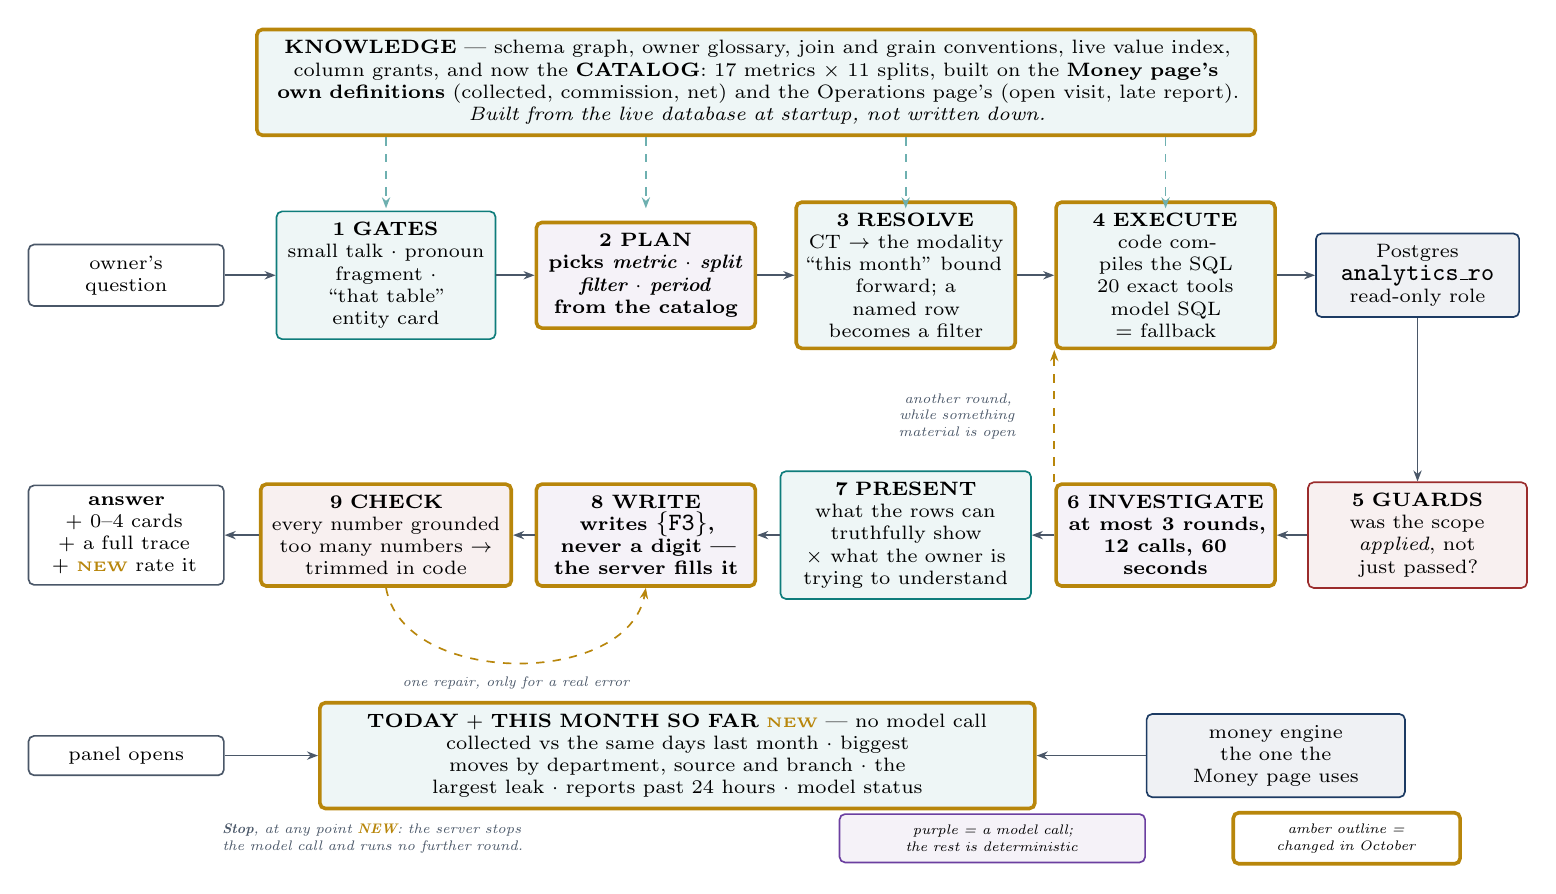
\begin{tikzpicture}[x=1cm,y=1cm, every node/.style={font=\scriptsize}]

\node[detbox, changed, text width=124mm] at (8.0,2.45)
  {\textbf{KNOWLEDGE} --- schema graph, owner glossary, join and grain conventions, live value index, column grants,
   and now the \textbf{CATALOG}: 17 metrics $\times$ 11 splits, built on the \textbf{Money page's own definitions}
   (collected, commission, net) and the Operations page's (open visit, late report).\\
   \scriptsize\itshape Built from the live database at startup, not written down.};

\node[box,      text width=22mm] (q)    at (0.0,  0) {owner's\\question};
\node[detbox,   text width=25mm] (gate) at (3.3,  0) {\textbf{1 GATES}\\small talk $\cdot$ pronoun\\fragment $\cdot$ ``that table''\\entity card};
\node[modelbox, changed, text width=25mm] (plan) at (6.6,  0) {\textbf{2 PLAN}\\picks \emph{metric $\cdot$ split}\\\emph{filter $\cdot$ period}\\from the catalog};
\node[detbox,   changed, text width=25mm] (res)  at (9.9,  0) {\textbf{3 RESOLVE}\\CT $\to$ the modality\\``this month'' bound\\forward; a named row\\becomes a filter};
\node[detbox,   changed, text width=25mm] (exe)  at (13.2, 0) {\textbf{4 EXECUTE}\\code compiles the SQL\\20 exact tools\\model SQL = fallback};
\node[databox,  text width=23mm] (db)   at (16.4, 0) {Postgres\\\code{analytics\_ro}\\read-only role};

\node[guardbox, text width=25mm] (grd)  at (16.4,-3.3) {\textbf{5 GUARDS}\\was the scope\\\emph{applied}, not\\just passed?};
\node[modelbox, changed, text width=25mm] (inv)  at (13.2,-3.3) {\textbf{6 INVESTIGATE}\\at most 3 rounds,\\12 calls, 60 seconds};
\node[detbox,   text width=29mm] (cap)  at (9.9, -3.3) {\textbf{7 PRESENT}\\what the rows can truthfully show\\$\times$ what the owner is\\trying to understand};
\node[modelbox, changed, text width=25mm] (wr)   at (6.6, -3.3) {\textbf{8 WRITE}\\writes \code{\{F3\}},\\never a digit ---\\the server fills it};
\node[guardbox, changed, text width=29mm] (chk)  at (3.3, -3.3) {\textbf{9 CHECK}\\every number grounded\\too many numbers $\to$\\trimmed in code};
\node[box,      text width=22mm] (out)  at (0.0, -3.3) {\textbf{answer}\\$+$ 0--4 cards\\$+$ a full trace\\$+$ \new{} rate it};

\foreach \x in {3.3,6.6,9.9,13.2} \draw[flow, dashed, draw=teal!60] (\x,1.75) -- (\x,0.85);

\draw[flow](q)--(gate); \draw[flow](gate)--(plan); \draw[flow](plan)--(res);
\draw[flow](res)--(exe); \draw[flow](exe)--(db);
\draw[flow](db)--(grd);
\draw[flow](grd)--(inv); \draw[flow](inv)--(cap); \draw[flow](cap)--(wr);
\draw[flow](wr)--(chk); \draw[flow](chk)--(out);

\draw[backflow] (inv.north west) -- node[lbl,left=0.5mm,text width=21mm]{another round, while something material is open} (exe.south west);
\draw[backflow] (chk.south) to[out=280,in=260] node[lbl,below=0.5mm]{one repair, only for a real error} (wr.south);

% the second lane: no model at all
\node[box, text width=22mm] (open) at (0.0,-6.1) {panel opens};
\node[detbox, changed, text width=88mm] (dig) at (7.0,-6.1)
  {\textbf{TODAY $+$ THIS MONTH SO FAR} \new{} --- no model call\\
   collected vs the same days last month $\cdot$ biggest moves by department, source and branch $\cdot$
   the largest leak $\cdot$ reports past 24 hours $\cdot$ model status};
\node[databox, text width=30mm] (eng) at (14.6,-6.1) {money engine\\the one the Money page uses};
\draw[flow](open)--(dig); \draw[flow](eng)--(dig);

\node[lbl, text width=60mm, anchor=west] at (0.0,-7.15)
  {\textbf{Stop}, at any point \new{}: the server stops the model call and runs no further round.};
\node[modelbox, text width=36mm, font=\tiny\itshape] at (11.0,-7.15)
  {purple = a model call; the rest is deterministic};
\node[box, changed, text width=26mm, font=\tiny\itshape] at (15.5,-7.15)
  {amber outline = changed in October};
\end{tikzpicture}
\end{fitpic}

\vspace{-2pt}
{\footnotesize\color{slate}\textbf{Cost of that:} 2 model calls and about 4--6 seconds for a figure (plan, then write). An open
question is 2--6 calls. The hard ceiling is 60 seconds and 12 calls, down from 180 seconds, and the answer must say so if it hits it.}

\vspace{4pt}
\hd{What we upgraded}
\vspace{-6pt}

{\footnotesize
\begin{tabular}{@{}L{2.5cm}L{6.6cm}L{8.2cm}@{}}
\toprule
\textbf{Upgrade} & \textbf{What was wrong} & \textbf{What it does now}\\
\midrule
\textbf{Catalog first} & The model wrote raw SQL in \was{50\%} of steps and \was{29\%} of those failed. ``give me cost'' took
 \was{31 calls}. & The model picks metric, split, filter and period; code compiles the SQL. Free SQL is only the fallback, now 4\% of steps.\\
\textbf{The Money page's numbers} & Pulse had its own revenue and commission formulas, so its totals disagreed with the Money page. &
 Collected, commission and net come from the same money engine. Checked equal to the rupee for yesterday, month to date and 30 days.\\
\textbf{Figures by reference} & The writer typed numbers. \was{15 of 31} answers needed a second, rewrite call. &
 The writer writes \code{\{F3\}}; the server fills in the value. A figure can only be one that a step measured.\\
\textbf{This month so far} & Nothing appeared until the owner asked a question. & A digest card with no model call:
 collected against the same days last month, the biggest moves, the largest leak and late reports.\\
\textbf{Stop} & The cancel signal fired 2\,ms into every request (Node 20), so Stop never stopped and keep-alives never went out. &
 Stop, or closing the panel, cancels the server work and the model call.\\
\textbf{Model status} & When the DeepSeek credit ran out, questions just failed. & The account is checked with a free call, at most every 10 minutes;
 the panel says when the model is down, and \code{/health} goes red.\\
\textbf{Thumbs up / down} & No way to know whether an answer was any good. & Every answer can be rated, with a note. It lands in the audit log.\\
\textbf{Same rules as the pages} & Late reports \was{349} against the Operations page's \was{13}; dues followed a different rule from the Money page; the Kidcare branches were left out. &
 Dues, late reports and branches follow the Money and Operations pages: 13 = 13.\\
\textbf{Bugs the benchmark found} & Splits silently cut at 200 rows (wrong ``most repeating customer''); ``CT'' read as Clotting Time;
 ``this month'' bound to last month; ``name him'' lost the row. & All fixed. Each question that caught one stays in the benchmark.\\
\textbf{A real benchmark} & 29 invented questions, scored by whether failure flags were absent. &
 41 of the owner's own questions, typos and all. Truth computed live from the money engine; 8 held out; the judge tests itself (71/71).\\
\bottomrule
\end{tabular}}

\clearpage

% =====================================================================
% PAGE 2 --- what it bought
% =====================================================================
{\color{navy}\Large\bfseries How it made things better}\hfill{\color{slate}\small page 2 of 3}\\[2pt]
{\color{mist}\hrule height 1.2pt}

\vspace{4pt}
{\footnotesize \textbf{Before} is September's production traces of the owner's real questions. \textbf{After} is the new benchmark
built from those same questions, run on 7 October against the live database. Every figure below was measured, not estimated.}

\vspace{4pt}
{\footnotesize
\begin{tabular}{@{}L{6.2cm}L{5.2cm}L{5.4cm}@{}}
\toprule
\textbf{Measure} & \textbf{Before (Sep)} & \textbf{After (Oct)}\\
\midrule
Model calls per question, median & \was{7} (mean 11) & \up{2}\\
Steps where the model wrote raw SQL & \was{50\%}, and 29\% of those failed & \up{4\%}\\
Most model calls on one question & \was{31} & \up{6}\\
Figures typed into the answer by the model & \was{all of them}; 48\% of answers then needed a rewrite call & \up{none}: the server fills them in\\
Time to answer, median & \was{23 s} & \up{6.6 s}\\
Time to answer, 90th percentile & \was{43 s} & \up{22 s}\\
\midrule
``give me cost'' & \was{31 calls, 43 s}, 13 model-written queries & \up{3 calls, 5 s}\\
``if the CT machine costs me 50 lakh, how long to pay back'' & \was{12--16} model-written queries per attempt & \up{5 calls, 22 s}\\
``which doctor is not sending much'' & \was{20 calls, 101 s} (first October run) & \up{4 calls, 22 s}\\
``read all the reasons for discounts'' & \was{12 calls, 53 s} (first October run) & \up{6 calls, 28 s}\\
``which test is heavily discounted'' & \was{11 calls, 38 s} (first October run) & \up{2 calls, 6 s}\\
\midrule
Collected, commission, CT collected vs the Money page & different formulas, different totals & \up{equal to the rupee} (yesterday, month to date, 30 days)\\
Reports past 24 hours vs the Operations page & \was{349} vs 13 & \up{13 = 13}\\
Splits longer than 200 rows & \was{silently cut}; ranks wrong & \up{complete}\\
\midrule
Benchmark, figures and lists & --- (29 invented questions) & \up{24/25} \quad(first full pass: 18/24)\\
Benchmark, open questions & --- & \up{7/8}\\
Benchmark, held out (never tuned on) & --- & \up{7/8}\\
Cost per question & \was{about \$0.04} (estimated from traces) & \up{under \$0.001} (\$0.03 for all 41, measured)\\
\bottomrule
\end{tabular}}

\vspace{6pt}
{\footnotesize\color{slate}\textbf{The three misses in that run.} Two were bugs, fixed since and re-run: the ``ct'' inside
``CT-BRAIN PLAIN'' was also read as \emph{every CT scan}, losing \rs{4,400} of orders; and ``which reports take the longest''
asked for turnaround by test, which has no catalog shape, and was not handed to SQL. The third gave dues by age correctly
but never stated their total.}

\vspace{4pt}
{\footnotesize\color{slate}Why it is faster and cheaper at the same time: a catalog step costs no model call and cannot fail
to compile, so the plan that used to spend 13 calls writing and repairing SQL now spends none. The latency that is left is
the two model round trips.}

\vspace{10pt}
\hd{The three things still wrong in September --- where they stand}
\vspace{-2pt}

\begin{fitpic}
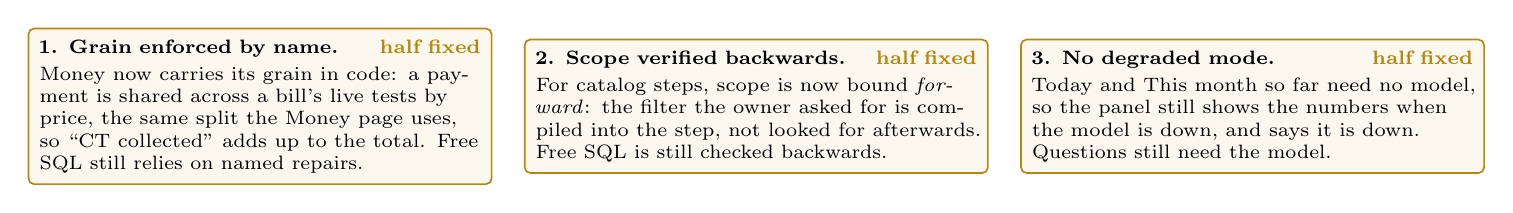
\begin{tikzpicture}[every node/.style={font=\scriptsize}]
\node[box, draw=amber, fill=amber!6, text width=56mm, align=left] (a)
 {\textbf{1. Grain enforced by name.} \hfill{\color{amber}\bfseries half fixed}\\[2pt]
  Money now carries its grain in code: a payment is shared across a bill's live tests by price, the same split the
  Money page uses, so ``CT collected'' adds up to the total. Free SQL still relies on named repairs.};
\node[box, draw=amber, fill=amber!6, text width=56mm, align=left, right=4mm of a] (b)
 {\textbf{2. Scope verified backwards.} \hfill{\color{amber}\bfseries half fixed}\\[2pt]
  For catalog steps, scope is now bound \emph{forward}: the filter the owner asked for is compiled into the step,
  not looked for afterwards. Free SQL is still checked backwards.};
\node[box, draw=amber, fill=amber!6, text width=56mm, align=left, right=4mm of b] (c)
 {\textbf{3. No degraded mode.} \hfill{\color{amber}\bfseries half fixed}\\[2pt]
  Today and This month so far need no model, so the panel still shows the numbers when the model is down, and says
  it is down. Questions still need the model.};
\end{tikzpicture}
\end{fitpic}

\vspace{8pt}
\hd{Found in the data along the way}
\vspace{-4pt}
{\footnotesize
\begin{itemize}[leftmargin=12pt,itemsep=1pt,topsep=1pt]
\item One bill is marked PAID but still has \rs{800} open, so it is missing from dues on both Pulse and the Money page.
\item One referring doctor is stored as two records, which splits their referrals in two in every ranking.
\item The Kidcare branches are now counted, because the Money page counts them. If they are test branches, both should drop them together.
\end{itemize}}

\vfill
{\scriptsize\color{slate}Before: production traces, September 2026, and the first October benchmark run where marked. After:
\code{pulse-real.ts} on 7 October 2026, figures compared with the money engine at run time. Raw results stay out of git (they name patients).}

\clearpage

% =====================================================================
% PAGE 3 --- what is next
% =====================================================================
{\color{navy}\Large\bfseries What we upgrade next, and what we expect}\hfill{\color{slate}\small page 3 of 3}\\[2pt]
{\color{mist}\hrule height 1.2pt}

\vspace{6pt}
{\footnotesize
\begin{tabular}{@{}L{3.3cm}L{5.0cm}L{4.6cm}L{4.0cm}@{}}
\toprule
\textbf{Next} & \textbf{Why} & \textbf{What we expect} & \textbf{How we will know}\\
\midrule
\textbf{Every question 3 times} & One run hides a model that passes once and fails on the rerun. &
 At least 95\% of questions pass all three runs. & pass-all against pass-any in the benchmark.\\
\textbf{Morning digest on WhatsApp} & The owner should see the numbers without opening the portal. &
 One message a day with the same lines as the card. & Meta template approved; delivered and read rates.\\
\textbf{Thumbs-down becomes a test} & Real failures are the questions worth testing. &
 Each one reviewed weekly and added with a computed truth. & The benchmark grows and its pass rate holds.\\
\textbf{Close the catalog gaps} & 10 of 70 real questions fit no catalog entry, and turnaround by test and report type are still missing. &
 Model-written SQL under 5\% of steps. & Its share in the benchmark and the production log.\\
\textbf{Remember what was said} & ``The machine costs 50 lakh'' and ``leave out JGG'' must be repeated today. &
 Follow-ups reuse the figures and filters the owner stated. & New chain cases in the benchmark.\\
\textbf{Grain and scope for free SQL} & The other half of the first two September problems. &
 Free SQL carries the same grain and scope as a catalog step. & No named repair left in the code.\\
\textbf{Answers with no model} & The third September problem, finished. & A figure question answered from the catalog when the model is down. &
 The benchmark run with the model switched off.\\
\bottomrule
\end{tabular}}

\vspace{10pt}
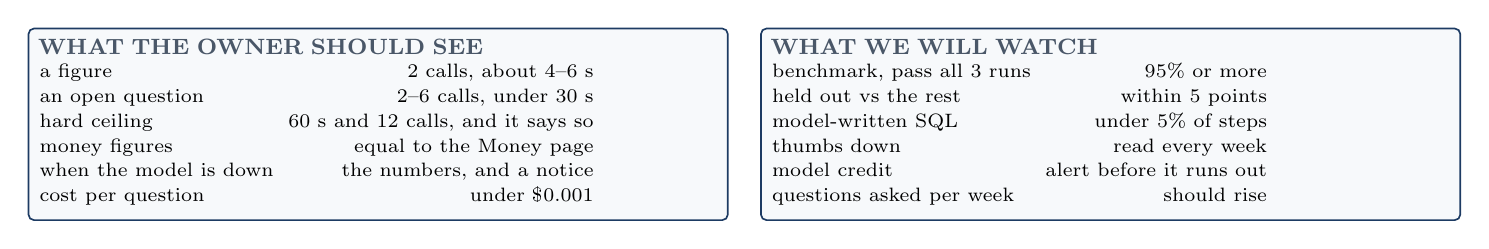
\begin{tikzpicture}[every node/.style={font=\footnotesize}]
\node[box, draw=navy, fill=paper, text width=86mm, align=left] (n1)
 {\shd{WHAT THE OWNER SHOULD SEE}
  \scriptsize
  \begin{tabular}{@{}l@{\ \ }r@{}}
  a figure & 2 calls, about 4--6 s\\
  an open question & 2--6 calls, under 30 s\\
  hard ceiling & 60 s and 12 calls, and it says so\\
  money figures & equal to the Money page\\
  when the model is down & the numbers, and a notice\\
  cost per question & under \$0.001\\
  \end{tabular}};
\node[box, draw=navy, fill=paper, text width=86mm, align=left, right=4mm of n1] (n2)
 {\shd{WHAT WE WILL WATCH}
  \scriptsize
  \begin{tabular}{@{}l@{\ \ }r@{}}
  benchmark, pass all 3 runs & 95\% or more\\
  held out vs the rest & within 5 points\\
  model-written SQL & under 5\% of steps\\
  thumbs down & read every week\\
  model credit & alert before it runs out\\
  questions asked per week & should rise\\
  \end{tabular}};
\end{tikzpicture}

\vspace{10pt}
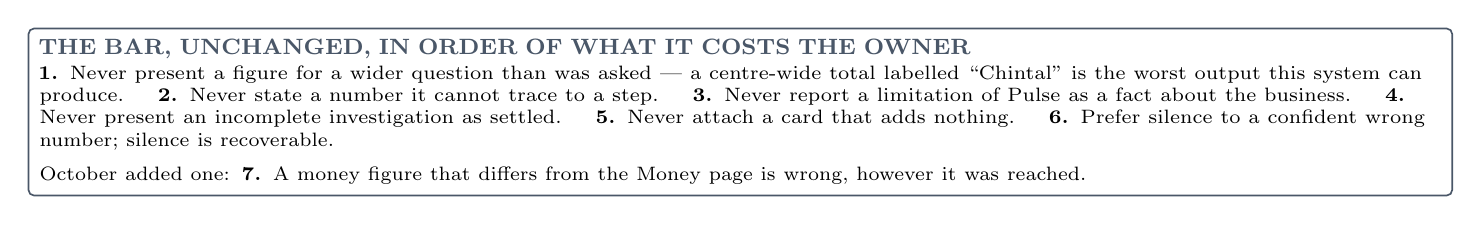
\begin{tikzpicture}
\node[box, draw=slate, fill=white, text width=178mm, align=left, font=\footnotesize]
 {\shd{THE BAR, UNCHANGED, IN ORDER OF WHAT IT COSTS THE OWNER}
  \scriptsize
  \textbf{1.} Never present a figure for a wider question than was asked --- a centre-wide total labelled
  ``Chintal'' is the worst output this system can produce. \quad
  \textbf{2.} Never state a number it cannot trace to a step. \quad
  \textbf{3.} Never report a limitation of Pulse as a fact about the business. \quad
  \textbf{4.} Never present an incomplete investigation as settled. \quad
  \textbf{5.} Never attach a card that adds nothing. \quad
  \textbf{6.} Prefer silence to a confident wrong number; silence is recoverable.\\[3pt]
  October added one: \textbf{7.} A money figure that differs from the Money page is wrong, however it was reached.};
\end{tikzpicture}

\vfill
{\scriptsize\color{slate}The security boundary is unchanged: \code{analytics\_ro}, read-only, column grants, eight-second timeout,
owner-only and audited. October added one column grant (\code{TestOrder.noReportAt}) so late reports can match the Operations page.
The September overview and \texttt{docs/pulse-architecture.pdf} (50 pp) still describe everything not listed here.}

\end{document}
